\documentclass[8pt]{beamer}
\usefonttheme[onlymath]{serif}


\setbeamertemplate{frametitle}{%
  \vskip1ex
  \usebeamerfont{frametitle}%
  \insertsubsectionhead\par        %  ← 원하는 대로 변경 가능
  \vskip1ex
  \hrule                             % 밑줄(선택)
}

% 테마 선택 (선택 사항)
% \usetheme{Madrid} % 기본 테마, 다른 테마 사용 가능
% \font{serif}
\usepackage{amsfonts}
\usepackage{amssymb}
\usepackage[T1]{fontenc} % To use combination of textbf, textit


% \setcounter{MaxMatrixCols}{20}

% (필요한 패키지들)
% \usepackage{amsthm}
\setbeamertemplate{theorems}[numbered]  % 정리, 정의 등에 번호를 달아줌

% \theoremstyle{plain} % insert bellow all blocks you want in italic
% \newtheorem{theorem}{Theorem}[section] % to number according to section
% 
% \theoremstyle{definition} % insert bellow all blocks you want in normal text
% \newtheorem{definition}{Definition}[section] % to number according to section
% \newtheorem*{idea}{Proof idea} % no numbered block
\usepackage{tcolorbox}

% 필요할 경우 패키지 추가
\usepackage{graphicx} % 이미지 삽입을 위한 패키지
\usepackage{amsmath}   % 수식 사용
\usepackage{hyperref}  % 하이퍼링크 추가
\usepackage{cleveref}
\usepackage{multicol}  % 여러 열 나누기
\usepackage{ulem} % 취소선 및줄 나누기



\newcommand{\mrm}[1]{\mathrm{#1}}
\newcommand{\mbb}[1]{\mathbb{#1}}
\newcommand{\mb}[1]{\mathbf{#1}}
\newcommand{\mc}[1]{\mathcal{#1}}
\newcommand{\tb}[1]{\textbf{#1}}
\newcommand{\ti}[1]{\textit{#1}}
\newcommand{\mypois}[1]{\operatorname{Pois}(#1)}

\newcommand{\mybin}[2]{\operatorname{Bin}\!\left(#1,#2\right)}
\newcommand{\mytoinf}[1]{#1 \rightarrow \infty}
\newcommand{\myexp}[1]{\exp{\left(#1\right)}}
\newcommand{\myunif}[2]{\operatorname{Unif}\!\left(#1, #2\right)}
\newcommand{\mygeom}[1]{\operatorname{Geom}\!\left(#1\right)}
\newcommand{\myexpo}[1]{\operatorname{Expo}\!\left(#1\right)}
\newcommand{\abs}[1]{\left\lvert #1 \right\rvert}
\newcommand{\expec}[1]{\operatorname{E}\left[ #1 \right]}
\newcommand{\myvar}[1]{\operatorname{Var}\left[#1\right]}
\newcommand{\myskew}[1]{\operatorname{Skew}\!\left[#1\right]}


% 발표 제목, 저자, 날짜 설정
\title{Probability}
\author{Gwanwoo Choi}
% \date{}

\begin{document}
% 표지 슬라이드
\begin{frame}
    \titlepage
\end{frame}

% % 목차 슬라이드
% \begin{frame}
%     \frametitle{Table of Contents}
%     \tableofcontents
% \end{frame}

\subsection{Summaries of a distribution}

\begin{frame}
    \frametitle{Table of Contents}
    \tableofcontents[currentsubsection]
\end{frame}


\begin{frame}{a}
    \begin{definition}[Median]
        We say that $c$ is a \tb{median} of a random variable $X$ if $P(X\leq c) \geq 1/2$ and $P(X \geq c) \geq 1/2$. (The simplest way this can happen is if the CDF of $X$ hits $1/2$ exactly at $c$, but we know that some CDFs have jumps.)
    \end{definition}

    \begin{definition}[Mode]
        For a discrete r.v. $X$, we say that $c$ is a \tb{mode} of $X$ if it maximizes the PMF: $P(X=c) \geq P(X = x), \forall x$. For a continuous r.v. $X$ with PDF $f$, we say that $c$ is a mode if it maximizes the PDF: $f(c) \geq f(x), \forall x$.
    \end{definition}

    \begin{itemize}
        \item The median and mode of an r.v. depend only on its \ti{distribution}.
        \item A distribution can have multiple medians and multiple modes.
    \end{itemize}

    \begin{figure}
        \centering
        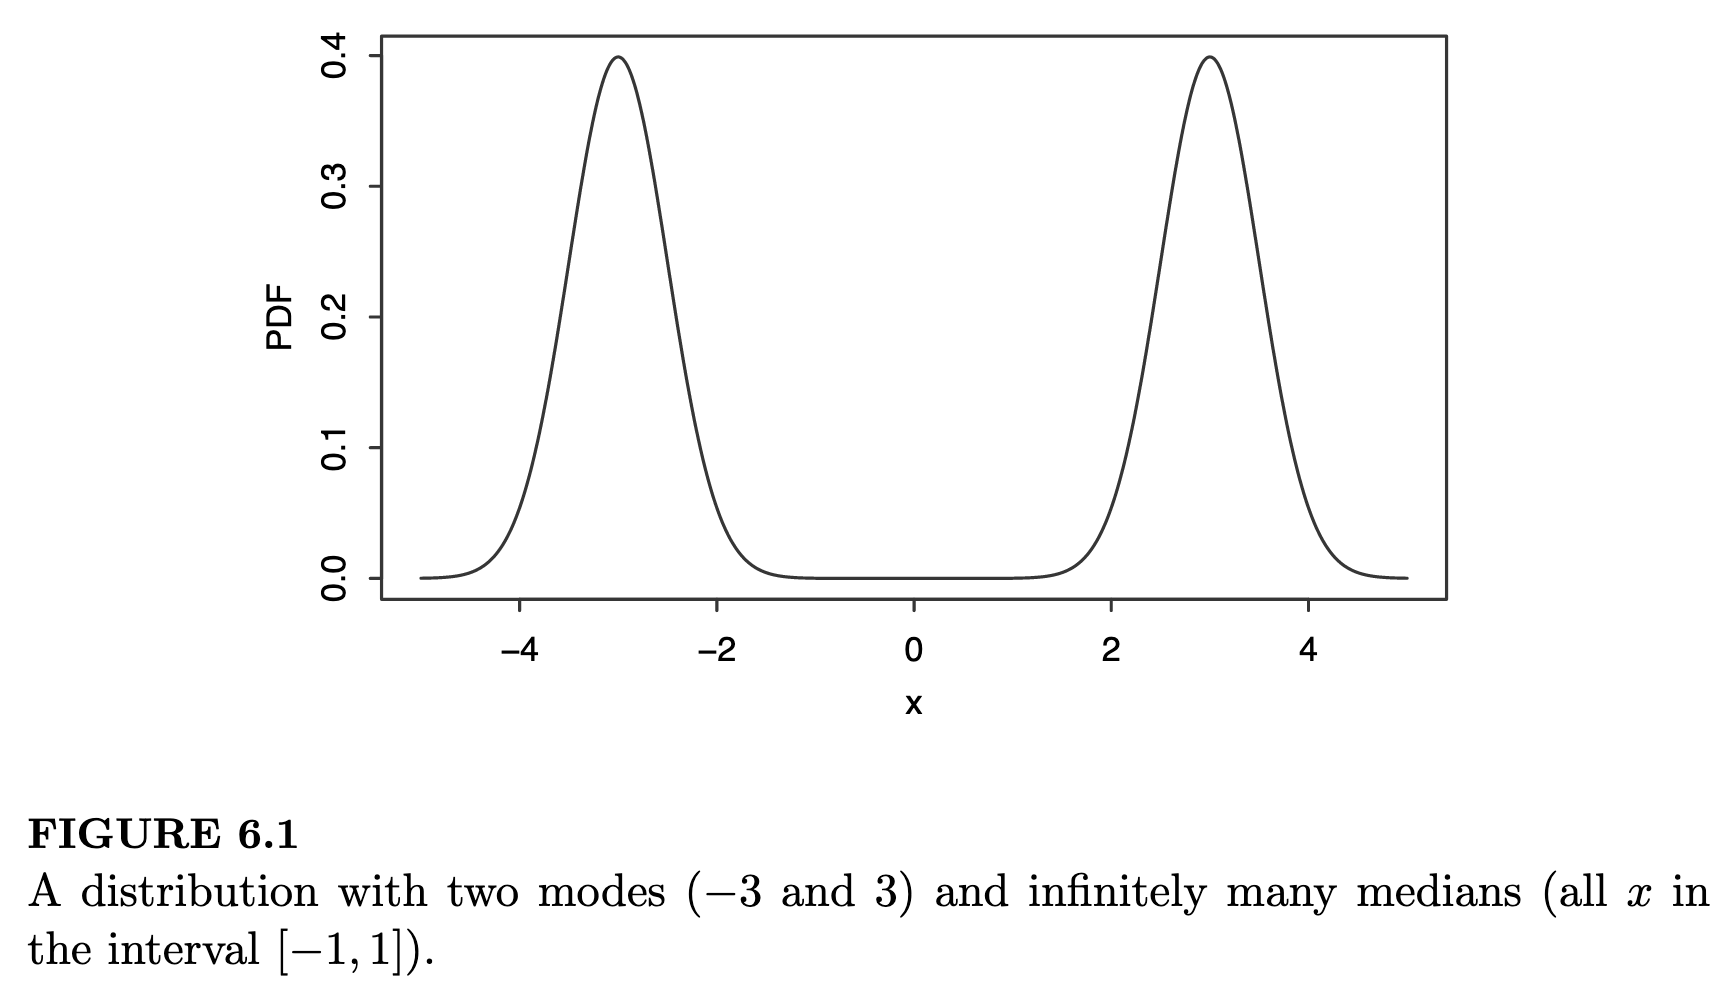
\includegraphics[width=0.55\textwidth]{fig1.png}
    \end{figure}
\end{frame}

\begin{frame}{a}
    \begin{example}[Mean, median, and mode for salaries]
        A certain company has $100$ employees. Let $s_1, s_2, \cdots, s_{100}$ be their salaries, sorted in increasing order. Let $X$ be the salary of a randomly selected employee (chosen uniformly). What is the most useful one-number summary of the salary data?
    \end{example}

    \begin{itemize}
        \item mode
        \begin{itemize}
            \item If the salaries are all different, then there exists $100$ different modes. 
            \item If there are only a few possible salaries in the company, the mode becomes more useful.
            \item But it could be also bad situation in such case. For example, 34 people receive salary $a$, 33 receive salary $b$ and 33 receive receive salary $c$.
        \end{itemize}
        \item median 
        \begin{itemize}
            \item Each number $s_{50}$ and $s_{51}$ can be median number.
            \item Any number $m$ such that $s_{50} \leq m \leq s_{51}$ can becomes median ($\because P(X \leq m) \geq 1/2, P(X \geq m) \geq 1/2$)
            \item Usual convention is to choose $m = (s_{50}+s_{51})/2$
        \end{itemize}
        \item mean
        \begin{itemize}
            \item Mean is more sensitive than the median. Consider the situation salary of CEO has slightly changed.
            \item On the other hand, suppose that we want to know the total cost the company is paying for its employees' salaries. If we only know a mode or a median, we can't extract this information.
        \end{itemize}
    \end{itemize}
\end{frame}

\begin{frame}{a}
    Suppose that we are trying to guess what a not-yet-observed r.v. $X$ will be, by making a prediction $c$. The mean and the median both seem like natural guesses for $c$, but which is better? It depends on \tb{how "better"} is defined.

    \begin{theorem}
        Let $X$ be an r.v. with mean $\mu$, and let $m$ be a median of $X$.
        \begin{itemize}
            \item The value of $c$ that minimizes the mean squared error $E[(X-c)^2]$ is $c=\mu$.
            \item The value of $c$ that minimizes the mean absolute error $E[\vert X-c \vert]$ is $c=m$.
        \end{itemize}
    \end{theorem}

    \textit{Proof.} We will first prove a useful identity $E[(X-c)^2] = Var[X] + (\mu -c)^2$. This can be drived by $Var[X] = Var[X-c] = E[(X-c)^2] - E[X-c]^2 = E[(X-c)^2] - (\mu - c)^2$. Then we can see that $E[(X-c)^2]$ is convex for $c$ and has global minimum at $c = \mu$.

    \bigskip
    \textit{Proof.} We need to show that $\forall a, \expec{\abs{X-m}} \leq \expec{\abs{X-a}}$.
    Assume $m < a$. If $X \leq m$ then $\abs{X -a} - \abs{X - m} = a - X - (m - X) = a -m$ and if $X > m$ then $\abs{X-a} - \abs{X-m} \geq m - a$. Let define r.v. $Y = \abs{X-a} - \abs{X-m}$ and indicator r.v. $I$ for $X \leq m$ (so, $1-I$ is the indicator r.v. for $X>m$). Then
    \[
    \begin{aligned}
        \expec{Y} &= \expec{YI} + \expec{Y(1-I)} \geq (a-m)\expec{I} + (m-a)\expec{(1-I)} \\
        &= (a-m)P(X\leq m) + (m-a)P(X > m) = (a-m)\{2P(X\leq m) - 1\} \\
        &\geq 0
    \end{aligned}
    \]
    And this implies $\expec{\abs{X-m}}\leq \expec{\abs{X-a}}$

\end{frame}

\subsection{Moments}

\begin{frame}
    \frametitle{tableofcontents}
    \tableofcontents[currentsubsection]
\end{frame}

\begin{frame}{a}
    \begin{definition}[Kinds of moments]
        Let $X$ be an r.v. with mean $\mu$ and variance $\sigma^2$. For any positive integer $n$, the $n$th \tb{moment} of $X$ is $E[X^2]$, the $n$th \tb{central moment} is $\expec{(X-\mu)^2}$, and the $n$th \tb{standardized moment} is $\expec{\left(\frac{X-\mu}{\sigma}\right)^n}$. Throughout the previous sentence, "if it exists" is left implicit.
    \end{definition}

    \bigskip
    The term \ti{moment} is borrowed form physics.
    \begin{figure}
        \centering
        
\includegraphics[width=0.5\textwidth]{fig2.png}
    \end{figure}
    Let $X$ be a discrete r.v. with distinct possible values $x_1, \dots, x_n$, and imagine a pebble with mass $m_j = P(X=x_j)$ positioned at $x_j$ on a number line, for each $j$.
    $\expec{X} = \sum_{j=1}^n m_j x_j$ is called the \ti{center of mass} of the system, and $\myvar{X} = \sum_{j=1}^n m_j (x_j - \expec{X})^2$ is called the \ti{moments of inertia} about the center of mass.

\end{frame}

\begin{frame}{a}
    \begin{definition}[Skewness]
        The \tb{Skewness} of an r.v. $X$ with mean $\mu$ and variance $\sigma^2$ is the third standardized moment of $X$.
        \[
            \myskew{X} = \expec{\left(\frac{X-\mu}{\sigma} \right)^3}
        \]
    \end{definition}
    \begin{itemize}
        \item Skewness is not depend on the location $\mu$ or the scale $\sigma$ by standardizing.
    \end{itemize}
    Why skewness measures \ti{asymmetry}?

    \begin{definition}[Symmetry of an r.v.]
        We say that an r.v. $X$ has a \ti{symmetric distribution about} $\mu$ if $X - \mu$ has the same distribution as $\mu - X$. If $X$ is symmetric about $\mu$, then
        \[
            \expec{X} - \mu = \expec{X - \mu} = \expec{\mu - X} = \mu - \expec{X} \implies \mu = \expec{X}
        \]
        Also, $\mu$ also becomes median. $P(X-\mu \leq 0) = P(\mu - X \leq 0) \implies P(X \leq \mu) = P(X \geq \mu)$
        \[
        \begin{gathered}
            P(X \leq \mu) = 1 - P(X > \mu) \geq 1 - P(X \geq \mu) = 1- P(X \leq \mu) \\
            \implies P(X \leq \mu) \geq \frac{1}{2}, P(X \geq \mu) \geq \frac{1}{2}
        \end{gathered}
        \]
        inequation is used for discrete r.v.
    \end{definition}
\end{frame}


\begin{frame}{Moments}
    \begin{lemma}[Symmetry in terms of the PDF]
        Let $X$ be a continuous r.v. with PDF $f$. Then $X$ is symmetric about $\mu$ 
    \end{lemma}
\end{frame}



\end{document}